\section{MKA Overview}
\label{sec:background}

\subsection{General Structure of MKA}

IEEE 802.1AE (MACsec)~\cite{ieee8021ae} provides confidentiality, integrity, and replay protection for Ethernet frames on a per-hop basis. The associated key-management protocol, defined in IEEE 802.1X~\cite{ieee8021x}, is MACsec Key Agreement (MKA). MKA operates over the EAP over LAN (EAPoL) control plane and supports the following lifecycle:

\begin{enumerate}
  \item \textbf{Connectivity Association setup.} Participants share a \emph{Connectivity Association Key} (CAK) through pre-provisioning or through an EAP exchange. A Connectivity Association (CA) is formed among peers that share the same CAK.
  \item \textbf{MKAPDU exchange} Each party in CA periadically exchanges \emph{MACsec Key Agreement Protocol Data Units} (MKAPDUs) to establish and maintain the cryptographic state. MKAPDUs carry the Key Number (KN), Message Number (MN), and encrypted Secure Association Keys (SAKs)(For Keyserver) along with an Integrity Check Value (ICV).
  \item \textbf{Key Server election.} A Key Server is elected among CA members according to the protocol’s priority and tie-breaking rules. The elected Key Server is responsible for generating SAKs.
  \item \textbf{Key derivation.} Each participant independently derives a \emph{Key Encryption Key} (KEK) and an \emph{Integrity Check Value Key} (ICK) from the CAK using a key derivation function (KDF). KEK is used for protection of Secure Association Keys (SAKs), while ICK is used to compute an Integrity Check Value (ICV) for message authentication.
  \item \textbf{SAK distribution.} The Key Server generates a fresh SAK, encrypts it with the KEK, appends an Integrity Check Value (ICV) computed with the ICK, and distributes the resulting MKAPDU to the other members. Each receiver verifies the ICV, decrypts the SAK, and acknowledges receipt.
  \item \textbf{Rekey.} SAKs are periodically refreshed, either because of traffic thresholds or administrative policy. Rekeying follows the same structure as the initial distribution, but with incremented Key Number (KN) and Message Number (MN) values.
\end{enumerate}

The simplified tamarin-based protocol flow shown in Figure~\ref{fig:mka_flow} illustrates the simplified two-party MKA exchange between a Key Server and a Server that we analyse in this paper, using the exact variable names and state facts of our Tamarin model.

\begin{figure}[htbp]
\centering
\resizebox{!}{0.90\textheight}{%
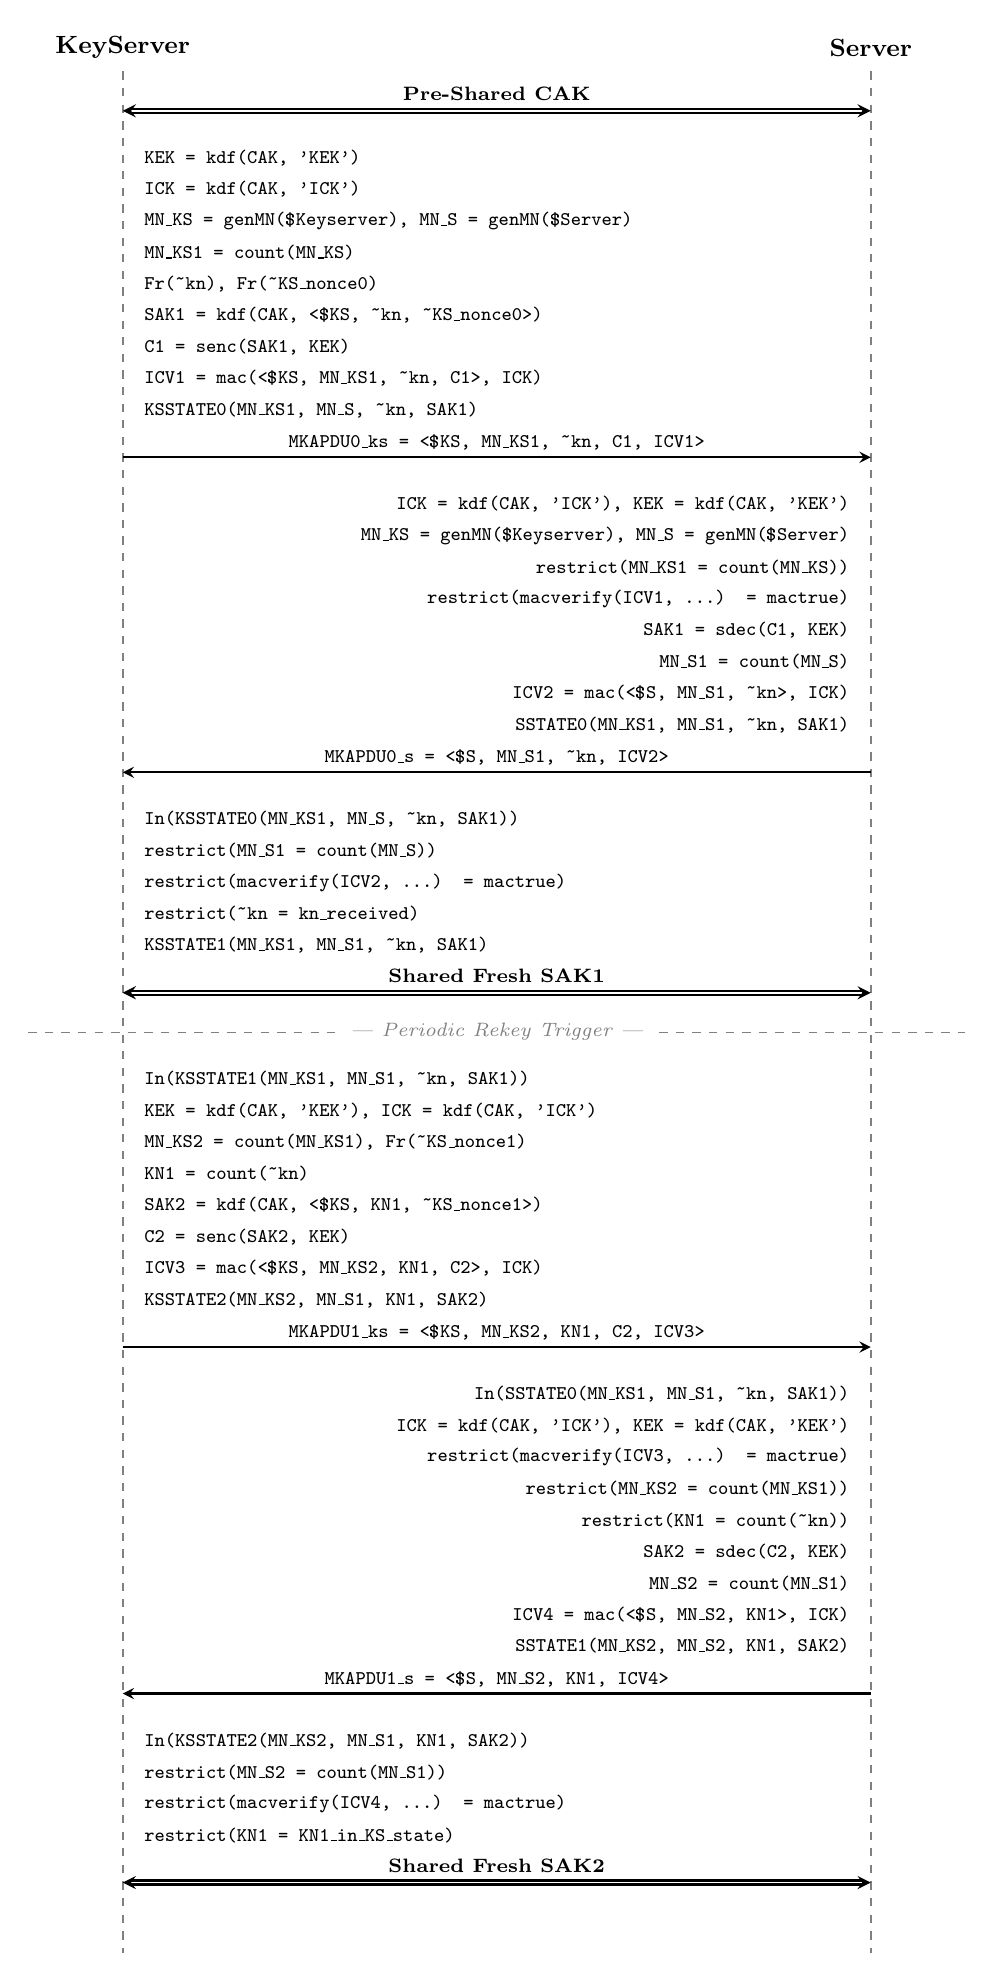
\begin{tikzpicture}[
  every node/.style={font=\scriptsize},
  arr/.style={->, >=stealth, thick},
  doublearr/.style={<->, >=stealth, thick, double},
  lbl/.style={font=\scriptsize\ttfamily, align=left},
  rlbl/.style={font=\scriptsize\ttfamily, align=right},
  msg/.style={font=\scriptsize\ttfamily, fill=white, inner sep=2pt}
]

% Lifelines
\def\KSx{0}
\def\Sx{9.5}

\node[font=\bfseries\small] (KS) at (\KSx, 0) {KeyServer};
\node[font=\bfseries\small] (S) at (\Sx, 0) {Server};

\draw[gray, dashed, thick] (\KSx, -0.3) -- (\KSx, -24.2);
\draw[gray, dashed, thick] (\Sx, -0.3) -- (\Sx, -24.2);

% Pre-shared CAK
\draw[doublearr] (\KSx, -0.8) -- node[above, font=\bfseries\scriptsize]{Pre-Shared CAK} (\Sx, -0.8);

% Initial - KeyServer Local
\node[lbl, anchor=west] at (\KSx+0.15, -1.4) {KEK = kdf(CAK, 'KEK')};
\node[lbl, anchor=west] at (\KSx+0.15, -1.8) {ICK = kdf(CAK, 'ICK')};
\node[lbl, anchor=west] at (\KSx+0.15, -2.2) {MN\_KS = genMN(\$Keyserver), MN\_S = genMN(\$Server)};
\node[lbl, anchor=west] at (\KSx+0.15, -2.6) {MN\_KS1 = count(MN\_KS)};
\node[lbl, anchor=west] at (\KSx+0.15, -3.0) {Fr(\textasciitilde kn), Fr(\textasciitilde KS\_nonce0)};
\node[lbl, anchor=west] at (\KSx+0.15, -3.4) {SAK1 = kdf(CAK, <\$KS, \textasciitilde kn, \textasciitilde KS\_nonce0>)};
\node[lbl, anchor=west] at (\KSx+0.15, -3.8) {C1 = senc(SAK1, KEK)};
\node[lbl, anchor=west] at (\KSx+0.15, -4.2) {ICV1 = mac(<\$KS, MN\_KS1, \textasciitilde kn, C1>, ICK)};
\node[lbl, anchor=west] at (\KSx+0.15, -4.6) {KSSTATE0(MN\_KS1, MN\_S, \textasciitilde kn, SAK1)};

% Msg 1
\draw[arr] (\KSx, -5.2) -- node[above, msg]{MKAPDU0\_ks = <\$KS, MN\_KS1, \textasciitilde kn, C1, ICV1>} (\Sx, -5.2);

% Initial - Server Local
\node[rlbl, anchor=east] at (\Sx-0.15, -5.8) {ICK = kdf(CAK, 'ICK'), KEK = kdf(CAK, 'KEK')};
\node[rlbl, anchor=east] at (\Sx-0.15, -6.2) {MN\_KS = genMN(\$Keyserver), MN\_S = genMN(\$Server)};
\node[rlbl, anchor=east] at (\Sx-0.15, -6.6) {restrict(MN\_KS1 = count(MN\_KS))};
\node[rlbl, anchor=east] at (\Sx-0.15, -7.0) {restrict(macverify(ICV1, \ldots) = mactrue)};
\node[rlbl, anchor=east] at (\Sx-0.15, -7.4) {SAK1 = sdec(C1, KEK)};
\node[rlbl, anchor=east] at (\Sx-0.15, -7.8) {MN\_S1 = count(MN\_S)};
\node[rlbl, anchor=east] at (\Sx-0.15, -8.2) {ICV2 = mac(<\$S, MN\_S1, \textasciitilde kn>, ICK)};
\node[rlbl, anchor=east] at (\Sx-0.15, -8.6) {SSTATE0(MN\_KS1, MN\_S1, \textasciitilde kn, SAK1)};

% Msg 2
\draw[arr] (\Sx, -9.2) -- node[above, msg]{MKAPDU0\_s = <\$S, MN\_S1, \textasciitilde kn, ICV2>} (\KSx, -9.2);

% Initial - KeyServer Confirm
\node[lbl, anchor=west] at (\KSx+0.15, -9.8) {In(KSSTATE0(MN\_KS1, MN\_S, \textasciitilde kn, SAK1))};
\node[lbl, anchor=west] at (\KSx+0.15, -10.2) {restrict(MN\_S1 = count(MN\_S))};
\node[lbl, anchor=west] at (\KSx+0.15, -10.6) {restrict(macverify(ICV2, \ldots) = mactrue)};
\node[lbl, anchor=west] at (\KSx+0.15, -11.0) {restrict(\textasciitilde kn = kn\_received)};
\node[lbl, anchor=west] at (\KSx+0.15, -11.4) {KSSTATE1(MN\_KS1, MN\_S1, \textasciitilde kn, SAK1)};

% Shared SAK1
\draw[doublearr] (\KSx, -12.0) -- node[above, font=\bfseries\scriptsize]{Shared Fresh SAK1} (\Sx, -12.0);

% Separator
\draw[dashed, gray] (-1.2, -12.5) -- (10.7, -12.5) node[midway, fill=white, font=\itshape\scriptsize]{--- Periodic Rekey Trigger ---};

% Rekey - KeyServer Local
\node[lbl, anchor=west] at (\KSx+0.15, -13.1) {In(KSSTATE1(MN\_KS1, MN\_S1, \textasciitilde kn, SAK1))};
\node[lbl, anchor=west] at (\KSx+0.15, -13.5) {KEK = kdf(CAK, 'KEK'), ICK = kdf(CAK, 'ICK')};
\node[lbl, anchor=west] at (\KSx+0.15, -13.9) {MN\_KS2 = count(MN\_KS1), Fr(\textasciitilde KS\_nonce1)};
\node[lbl, anchor=west] at (\KSx+0.15, -14.3) {KN1 = count(\textasciitilde kn)};
\node[lbl, anchor=west] at (\KSx+0.15, -14.7) {SAK2 = kdf(CAK, <\$KS, KN1, \textasciitilde KS\_nonce1>)};
\node[lbl, anchor=west] at (\KSx+0.15, -15.1) {C2 = senc(SAK2, KEK)};
\node[lbl, anchor=west] at (\KSx+0.15, -15.5) {ICV3 = mac(<\$KS, MN\_KS2, KN1, C2>, ICK)};
\node[lbl, anchor=west] at (\KSx+0.15, -15.9) {KSSTATE2(MN\_KS2, MN\_S1, KN1, SAK2)};

% Msg 3
\draw[arr] (\KSx, -16.5) -- node[above, msg]{MKAPDU1\_ks = <\$KS, MN\_KS2, KN1, C2, ICV3>} (\Sx, -16.5);

% Rekey - Server Local
\node[rlbl, anchor=east] at (\Sx-0.15, -17.1) {In(SSTATE0(MN\_KS1, MN\_S1, \textasciitilde kn, SAK1))};
\node[rlbl, anchor=east] at (\Sx-0.15, -17.5) {ICK = kdf(CAK, 'ICK'), KEK = kdf(CAK, 'KEK')};
\node[rlbl, anchor=east] at (\Sx-0.15, -17.9) {restrict(macverify(ICV3, \ldots) = mactrue)};
\node[rlbl, anchor=east] at (\Sx-0.15, -18.3) {restrict(MN\_KS2 = count(MN\_KS1))};
\node[rlbl, anchor=east] at (\Sx-0.15, -18.7) {restrict(KN1 = count(\textasciitilde kn))};
\node[rlbl, anchor=east] at (\Sx-0.15, -19.1) {SAK2 = sdec(C2, KEK)};
\node[rlbl, anchor=east] at (\Sx-0.15, -19.5) {MN\_S2 = count(MN\_S1)};
\node[rlbl, anchor=east] at (\Sx-0.15, -19.9) {ICV4 = mac(<\$S, MN\_S2, KN1>, ICK)};
\node[rlbl, anchor=east] at (\Sx-0.15, -20.3) {SSTATE1(MN\_KS2, MN\_S2, KN1, SAK2)};

% Msg 4
\draw[arr] (\Sx, -20.9) -- node[above, msg]{MKAPDU1\_s = <\$S, MN\_S2, KN1, ICV4>} (\KSx, -20.9);

% Rekey - KeyServer Confirm
\node[lbl, anchor=west] at (\KSx+0.15, -21.5) {In(KSSTATE2(MN\_KS2, MN\_S1, KN1, SAK2))};
\node[lbl, anchor=west] at (\KSx+0.15, -21.9) {restrict(MN\_S2 = count(MN\_S1))};
\node[lbl, anchor=west] at (\KSx+0.15, -22.3) {restrict(macverify(ICV4, \ldots) = mactrue)};
\node[lbl, anchor=west] at (\KSx+0.15, -22.7) {restrict(KN1 = KN1\_in\_KS\_state)};

% Shared SAK2
\draw[doublearr] (\KSx, -23.3) -- node[above, font=\bfseries\scriptsize]{Shared Fresh SAK2} (\Sx, -23.3);

\end{tikzpicture}%
}
\caption{Simplified two-party MKA protocol flow (initial session and rekey round) as specified in \texttt{MKA\_v10.spthy}. \$KS = KeyServer identity, \$S = Server identity, MN = Message Number counter, KN = Key Number counter.}
\label{fig:mka_flow}
\end{figure}